% This must be in the first 5 lines to tell arXiv to use pdfLaTeX, which is strongly recommended.
\pdfoutput=1
% In particular, the hyperref package requires pdfLaTeX in order to break URLs across lines.

\documentclass[11pt]{article}

% Remove the "review" option to generate the final version.
\usepackage[review]{ACL2023}

% Standard package includes
\usepackage{times}
\usepackage{latexsym}

% For proper rendering and hyphenation of words containing Latin characters (including in bib files)
\usepackage[T1]{fontenc}
% For Vietnamese characters
% \usepackage[T5]{fontenc}
% See https://www.latex-project.org/help/documentation/encguide.pdf for other character sets

% This assumes your files are encoded as UTF8
\usepackage[utf8]{inputenc}

% This is not strictly necessary, and may be commented out.
% However, it will improve the layout of the manuscript,
% and will typically save some space.
\usepackage{microtype}

% This is also not strictly necessary, and may be commented out.
% However, it will improve the aesthetics of text in
% the typewriter font.
\usepackage{inconsolata}
\usepackage{graphicx} %插入图片的宏包
\usepackage{float} %设置图片浮动位置的宏包
\usepackage{subfigure} %插入多图时用子图显示的宏包

% If the title and author information does not fit in the area allocated, uncomment the following
%
%\setlength\titlebox{<dim>}
%
% and set <dim> to something 5cm or larger.

\title{Comparing Different Keywords Extraction Methods}

% Author information can be set in various styles:
% For several authors from the same institution:
% \author{Author 1 \and ... \and Author n \\
%         Address line \\ ... \\ Address line}
% if the names do not fit well on one line use
%         Author 1 \\ {\bf Author 2} \\ ... \\ {\bf Author n} \\
% For authors from different institutions:
% \author{Author 1 \\ Address line \\  ... \\ Address line
%         \And  ... \And
%         Author n \\ Address line \\ ... \\ Address line}
% To start a seperate ``row'' of authors use \AND, as in
% \author{Author 1 \\ Address line \\  ... \\ Address line
%         \AND
%         Author 2 \\ Address line \\ ... \\ Address line \And
%         Author 3 \\ Address line \\ ... \\ Address line}


\author{Wuhao}
  % \texttt{wuhwa469@student.liu.se} \\}

\begin{document}
\maketitle
\begin{abstract}
  Key-words extraction is an important task in NLP fields, many advanced tasks are based on key-words extraction.
  In this project, TF-IDF, Keybert, TextRank and Yake will be compared. The dataset is from other NLP competitions
  and the evaluation is based on the f1-score. We found that Keybert and Yake are with the highest f1-score while
  TF-IDF is the most efficient method. Textrank is not flexible since it can not customize the number of keywords.
\end{abstract}

\section{Introduction}

Key-words detection is always an important task in many text applications. In this project, four methods will be discussed and compared.
The first methods are TF-IDF$\footnote{\url{https://en.wikipedia.org/wiki/Tf/$\%$E2/$\%$80$\%$93idf}}$, which basically calculates and compares
the frequency of a specific word in all the text data and one text data. A higher TF-IDF value means higher importance of this word to the text. 


\vspace{11pt}
  \noindent
Another model isknown as Yake\cite{yake1}\cite{yake2}\cite{yake3}. Yake can be considered as an extension of TF-IDF, this algorithm will calculate TF-IDF value and also cosine similarity, then a word graph will be 
constructed to obtain the weights of each candidate word. 

\vspace{11pt}
  \noindent
The third one is a self-supervised 
learning method called KeyBert \cite{keybert}. In this approach, document-level vector representations 
are extracted by BERT. Subsequently, word vectors are extracted for the N-gram words/phrases, and then, cosine similarity will be applied to find the most similar 
word/phrase to the document. Finally, the selected words will be identified as the words that best describe the entire document. 

\vspace{11pt}
  \noindent
Last Algorithm is TextRank\cite{textrank}.
The TextRank algorithm is a graph-based sorting algorithm. The workflows are as follows: putting text segmentation into several constituent units (e.g. sentences), 
building a node connection graph, using similarity between sentences as the edge Weights, calculating the TextRank value of the sentence through loop iterations, and finally extracting the sentences with high rankings 
and combine them into text summaries.

\subsection{Motivation}
The main purpose of this project is to explore the performance and characteristics of different models so that a reasonable choice of models can be made in practical scenarios. Keyword extraction is usually used as a base task for other natural language processing tasks, so the selection of an efficient model can help a lot to improve the overall task timeliness
\section{Related work}

Mohammad\text{-}Reza Feizi\text{-}Derakhshi\cite{bmo} used bert model to do key-phrase extraction. The bert model with graph-text-based embedding can reach a 0.70 f1-score. 
MingXi Zhang\cite{article33} tested the Textrank algorithm in many key-words extraction datasets, but they only have the precision as evaluation.
In 2018, Bijoyan Das and Sarit Chakraborty\cite{DBLP} used TF-IDF to grab keywords and use those keywords to do different tasks. In a classification task, they reach 96.83$\%$
accuracy. Shahzad Qaiser and Ramsha Ali \cite{234}used TF-IDF to find the words with the highest
relevance to the documents, they compared their rank results with the golden label but they did not mention evaluation scores like f1-score. SusieXi Rao, Piriyakorn Pirytamwong and Parijat Ghoshal \cite{rao} did experiment on different algorithms including textrank and keybert. They use k-means to help textrank clusterings and used a self-trained model as a keybert language model. The result show textrank is more time efficient than keybert but lower f1-score.

\section{Dataset}
The data set used in this project is Inspec \cite{inspec}. The language is English, and the original text is collected from scientific papers within computer
science fields. Below are the numeric features of the data.

\begin{center}
  \begin{tabular}{cccc}
      \hline
      N-docs& TG & TPD\\
      \hline
      2000&29230& 128.2\\
      
      \hline
      \end{tabular}
  \end{center}
  \noindent
  \textbf{N-docs} is the number of documents contained in the data, \textbf{TG} is the number
  of gold keywords in the dataset, \textbf{TPD} is an average number of tokens in each document.

   \begin{figure}[H] %H为当前位置,!htb为忽略美学标准,htbp为浮动图形
\centering %图片居中
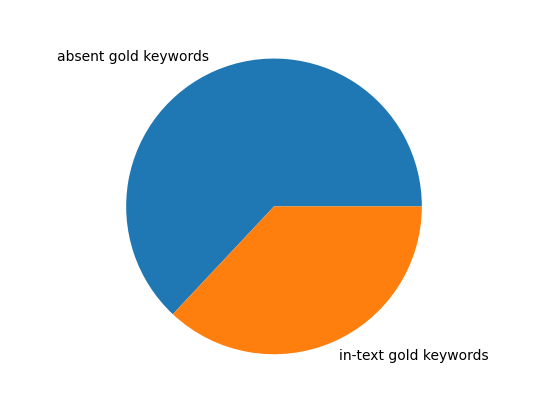
\includegraphics[width=0.55\textwidth]{pic/pie.png} %插入图片,[]中设置图片大小,{}中是图片文件名
\caption{Absent gold keywords} %最终文档中希望显示的图片标题
\label{Fig.main6} %用于文内引用的标签
\end{figure}
   \noindent
  The advantage of using this data is that the dataset contains only 2000 documents with an average number of tokens of 128. This means the training is less computational density than a huge dataset. But the dataset contains 37 percent golden keywords (see graph above) that are absent in the resource document, this will automatically lead to a lower recall rate.
  
  \section{Evaluation}
  In the competition \cite{augenstein-etal-2017-semeval} held by Association for Computational Linguistics in Vancouver, Canada,
  they use the f1-score to evaluate the results. In this project, all the model performances will be evaluated by f1-score in this project. The f1-score is more robust than accuracy.
  The f1-score can be calculated by:
  
  \begin{equation}
    \begin{aligned}
      f1 &= \frac{2}{recall^{-1}+precision^{-1}} \\
      &= \frac{2tp}{2tp+fp+fn}
      \end{aligned}
  \end{equation}

  \noindent
  Tp here means true positive, fp here means false positive and fn means false negative. In this project, \textbf{true positive} means if a gold key-word is predicted as a gold key-word,
  \textbf{false negative} means if a gold key-word is predicted as a non-gold key-word,\textbf{false positive}
  means if a non-gold keyword is predicted as a gold keyword.
  As mentioned before, this dataset contains an average of 37 percent golden keywords that are absent in the document, this means the false negative will be higher than 0.37. This will make the f1-score of each model lower than the usual dataset.
  \section{Experiment}
  In this section, the results of each method will be presented and discussed. TF-IDF, Keybert, and Yake support a customized number of keywords. We will select 5 benchmarks (10,12,16,18,20) to test each model's f1 score. The textrank methods implemented by spacy or summa do not support the number of keywords as a hyperparameter, so the results from two different implementations will be compared.
  \subsection{TF-IDF}
  For TF-IDF method, this project is referring to the spacy package$\footnote{\url{https://github.com/explosion/spaCy}}$. TF-IDF will calculate the frequency of a term showing up in a document(tf) and also ratio of how many documents contains the term(idf). A higher tf-idf value is supposed to imply a more important term.
  The results of TF-IDF method are as follows. N is the number of keywords that the model would extract, and f1 is the corresponding f1-score.
  \begin{figure}[H] %H为当前位置,!htb为忽略美学标准,htbp为浮动图形
\centering %图片居中
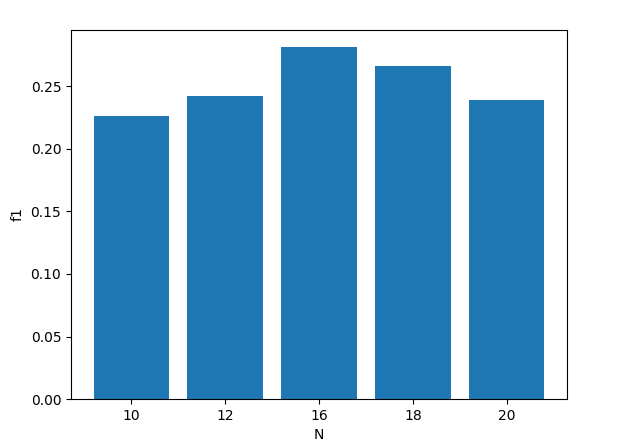
\includegraphics[width=0.52\textwidth]{pic/tfidf.png} %插入图片,[]中设置图片大小,{}中是图片文件名
\caption{TF-IDF results} %最终文档中希望显示的图片标题
\label{Fig.main5} %用于文内引用的标签
\end{figure}
  
  \subsection{Yake}
  For yake model, this project is referring to the official package$\footnote{\url{https://github.com/LIAAD/yake}}$. Yake is an unsupervised method, it will first find similar articles by calculating tf-idf and their cosine distance. With in those selected words, candidate words will be selected by calculating the global affinity graph. The keywords will be then selected by sorting candidate words according to global affinity graph value from high to low.
  The results of yake are as follows. N is the number of keywords that the model would extract, and f1 is the corresponding
  f1-score. Note that there are many other parameters that can be tuned, see the appendix for more details.
  \begin{figure}[H] %H为当前位置,!htb为忽略美学标准,htbp为浮动图形
\centering %图片居中
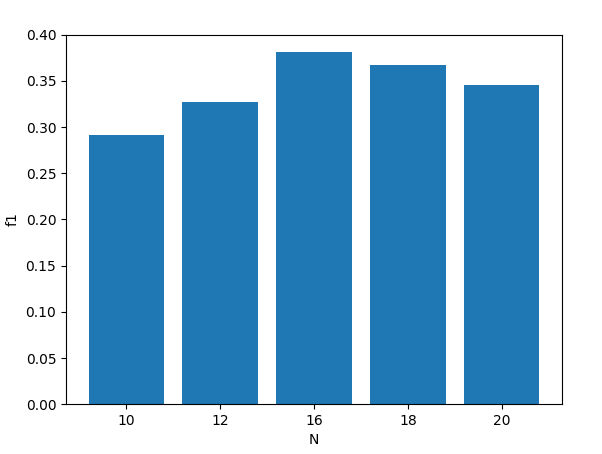
\includegraphics[width=0.52\textwidth]{pic/yake.png} %插入图片,[]中设置图片大小,{}中是图片文件名
\caption{Yake results} %最终文档中希望显示的图片标题
\label{Fig.main2} %用于文内引用的标签
\end{figure}
  
  \subsection{Keybert}
  For Keybert model, this project is referring to the official package$\footnote{\url{https://github.com/MaartenGr/KeyBERT}}$. Keybert uses bert skeleton. A pre-trained network will be applied to extract word vectors. Then N-gram will be calculated and compared will the document vector. Keywords will then be selected by sorting the cosine distance between the candidate word vector and the document.
  The results of Keybert are as follows. N is the number of keywords that the model would extract, and f1 is the corresponding
  f1-score. Note that there are many other parameters that can be tuned, see the appendix for more details.
  
  \begin{figure}[H] %H为当前位置,!htb为忽略美学标准,htbp为浮动图形
\centering %图片居中
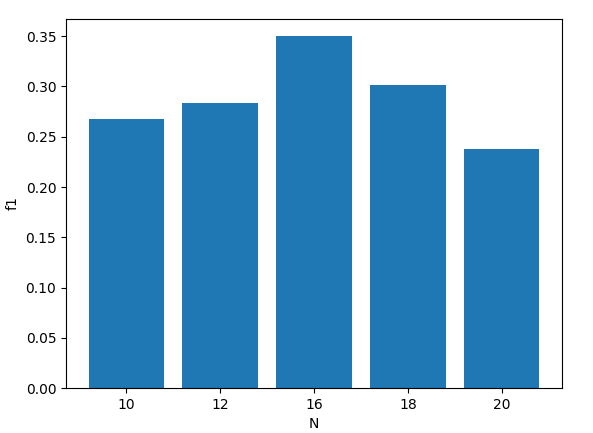
\includegraphics[width=0.52\textwidth]{pic/bert.png} %插入图片,[]中设置图片大小,{}中是图片文件名
\caption{Keybert results} %最终文档中希望显示的图片标题
\label{Fig.main4} %用于文内引用的标签
\end{figure}
  
  \subsection{Textrank}
  For the textrank model, this project is referring to two different implementations, one is summaNLP$\footnote{\url{https://github.com/summanlp/textrank}}$,
  another one is spacy $\footnote{\url{https://spacy.io/universe/project/spacy-pytextrank}}$. By partitioning the text into several component units (words, sentences) and building a graph model, and using a voting mechanism to rank the important components of the text, keyword extraction and digestion can be achieved using only the information of a single document itself. The Textrank algorithm does not
  offer "number of keywords" parameter, the results of two different implementations are as follows:
  
  \begin{center}
      \begin{tabular}{ccc}
          \hline
          implementations& summaNLP& Spacy\\
          \hline
          f1& 0.200& 0.179 \\
          \hline
      \end{tabular}
  \end{center}
  \noindent
  
  \section{Discussion}
  All the models have the highest f1 score when the number of keywords is 16. To clearly compare each model's performance, the highest f1 score of each model is selected below.
  \begin{figure}[H] %H为当前位置,!htb为忽略美学标准,htbp为浮动图形
\centering %图片居中
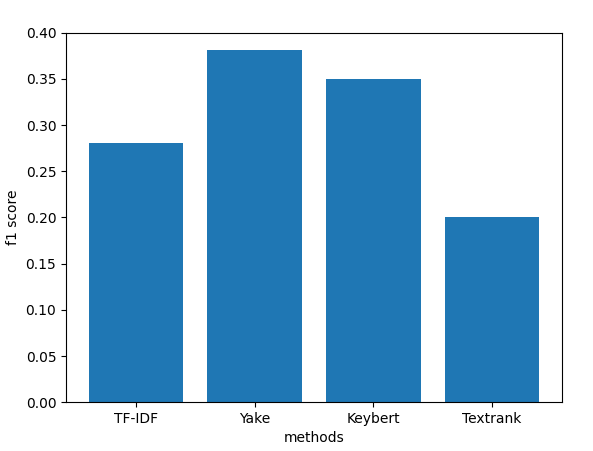
\includegraphics[width=0.52\textwidth]{pic/p1.png} %插入图片,[]中设置图片大小,{}中是图片文件名
\caption{Highest Score Of Each Model} %最终文档中希望显示的图片标题
\label{Fig.main2} %用于文内引用的标签
\end{figure}

    \vspace{11pt}
  \noindent
  Yake is based on TF-IDF, the weights of each word come from document-level statistics. But Yake considers more features than TF-IDF and the f1-score also reflects that Yake is more advanced than TF-IDF.
  
  \vspace{11pt}
  \noindent
  Keybert uses BERT to extract the word vectors and considers the similarity between words and documents. So, the result highly depends on which pre-trained network is used. 
  
  \vspace{11pt}
  \noindent
  Textrank is based on a graph algorithm. Like a transformer-based model, it will divide the text into different parts. The different
  thing is that Textrank will consider those elements as points and edges in a graph. Then a voting system will
  select the most important words.

  
  \section{Conclusion}
  From the experiment results, one can easily see that yake and keybert are much better than the other two methods. For this 
  dataset, every document contains an average of 15 golden keywords. And for textrank which does not receive the "number of keywords" parameter,
  the f1-score is lower because of too few key-words predictions. In this project, We also try to set "number of key-words = 5" for other
  models and the results are quite similar to textrank. In one word, the TF-IDF method is the fastest method among these four methods while keybert and yake have the highest f1-score.
  
\vspace{11pt}
  \noindent
   For simple keyword extraction like getting keywords from a paper, tf-idf value is enough since this scenario normally needs several single words to identify the research fields, and tf-idf method is the simplest method with the highest time efficiency. For more complex works where contextual information is needed like extracting keywords from a piece of news or a pice of product description, we need keybert, Yake, or textrank since those methods build a language model and take context into consideration. When it comes to key-phrase extraction, tf-idf methods can hardly work since this method has no representation of a phrase.
    
 \vspace{11pt}
  \noindent
  Note that in Inspec dataset, 37.7$\%$ of keywords do not show up in the text, which means the 'fn' in the f1-score is at least
  0.37. That is an important reason why all the models can not have a high f1-score.

  
  \vspace{11pt}
  \noindent
  The drawback of TF-IDF is obvious. TF-IDF method can only get every single keyword. When it comes
  to key phrase extraction(KPE), the TF-IDF method can not work. 
  
  \section{Future Work}
  In this project, the dataset semeval2017 \cite{augenstein-etal-2017-semeval} 
  , which contains key phrases, is also applied to all of these four models. We pick the same hyperparameters as in the Inspec datasets, but the length
  of a key phrase is set in a range from 1 to 4.
  \vspace{11pt}
  \begin{center}
      \begin{tabular}{ccccc}
          \hline
          models& TF-IDF& Keybert& TextRank& Yake\\
          \hline
          f1& 0.04& 0.13& 0.12& 0.15 \\
          \hline
      \end{tabular}
  \end{center}
  
  \noindent
  \vspace{11pt}
  
  Based on this project, there are multiple future tasks. The most important thing is to think about how can we use the TF-IDF method to predict key phrases. Maybe this can be achieved by combining the candidate keywords and re-calculate the weights.
  
   \noindent
  \vspace{11pt}
  Another thinking is about how to improve other models' f1-score in keyphrase extraction. Maybe this can be achieved by applying some pre-processing procedure or using a more advanced pre-trained word2vec model in keybert. There is also a possibility to ensemble different models and get more robust ensembled models. 
  
  \vspace{11pt}
  \noindent
  In the semeval-2017 competition, the highest team reach the f1-score of 0.68. It is a quite good result but is still
  far away from the practical usage standard.

  
  \bibliographystyle{acl_natbib}
  \bibliography{custom}

  \newpage
  \appendix
  \section{Appendices}

  \subsection{Hyperparameter}
  For Keybert
  \begin{center}
      \begin{tabular}{cccc}
          \hline
          hp& div&maxsum & model\\
          \hline
          value& 0.2& False& 'all-MiniLM-L6-v2' \\
          \hline
      \end{tabular}
  \end{center}
  \noindent
  For Yake
  \begin{center}
      \begin{tabular}{cccc}
          \hline
          hp& threshold& algorithm& Size\\
          \hline
          value&  0.9& 'seqm'& 1 \\
          \hline
      \end{tabular}
  \end{center}
    
\end{document}



